\documentclass{article}
\usepackage{amsmath}
\usepackage{amssymb}
\usepackage{graphicx}
\usepackage{hyperref}
\usepackage[version=4]{mhchem}


\begin{document}
As shown in the figure, \(A B C D\) is a parallelogram with \(A C / / B E . D E\) meets the extension of \(A C\) at \(F\); meets \(B E\) at \(E\). Prove: \(D F=\) FE.

Solution:
Extend \(D C\) to meet \(A E\) at \(M\).\\
\centering
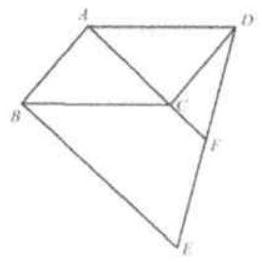
\includegraphics[width=\textwidth]{images/037.jpg}

Since \(A B / / D C, A B / / C M\).\\
We know that \(A C / / B E\), so \(A C / / B M\).


Therefore, \(A B M C\) is a parallelogram with \(A B=C M\).\\
Since \(A B C D\) is a parallelogram, \(A B=C D\).\\
Thus \(D C=C M\) and C is the midpoint of \(D M\).\\
\centering
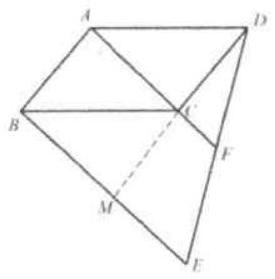
\includegraphics[width=\textwidth]{images/038(1).jpg}

Since \(C F / / M E\), it divides the line segment \(D E\) such that \(D F=F E\).\\

\end{document}
